\documentclass{article}
\usepackage[utf8]{inputenc}
\usepackage{amsmath}
\usepackage{amssymb}
\usepackage{graphicx}
\usepackage{hyperref}
\usepackage{tikz}
\usepackage{pgfplots}
\usepackage{float}
\usepackage{listings}
\usepackage{color}
\usepackage{bbm}
\usepackage{multirow}

\title{Reinforcement Learning \\ Exercise 4 - Solution}
\author{Jonathan Schnitzler - st166934 \\
Eric Choquet - st160996}
\date{\today}
\begin{document}
\maketitle
\section*{Task 1)}


\paragraph*{a) Advantages of Monte Carlo over dynamic programming}

\begin{enumerate}
    \item Does not require knowlegde of the environment $p(s'| s,a)$ and $r(s,a,s')$.
    \item Simulate experience via simulator (or real world)
    \item Can be updated every episode vs every state
\end{enumerate}

\paragraph*{b) Example for Monte Carlo to learn the value function (over DP)}

MC is preferable over DP when the distributions $p(s'|s, a)$ and $r(s,a,s')$ can not or only with very much effort be sampled. For example, in poker or blackjack, it is too complicated to model the distribution of the next state given the current state and action. In this case, MC can be used to learn the value function by simulating the experience of playing the game. This is especially useful when there is no model of the environment available.



\section*{Task 2)}

Programming task

\begin{figure}[H]
\centering
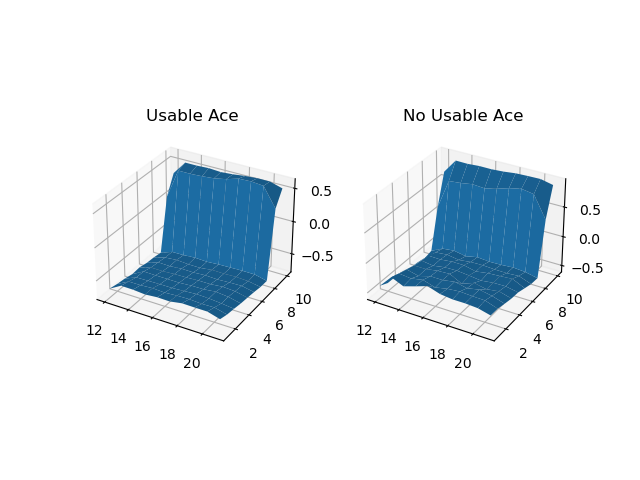
\includegraphics[width=\textwidth]{media/surface_plot.png}
\caption{Task 2b: Always hit till 20 with maxiter = 1000000}
\label{fig:}
\end{figure}
The state space of blackjack consists of the values 12 to 21 for the player and 1 to 10 for the dealer. Further an ace can be used or not. The action space consists of two actions: hit or stick. 
The policy which Monte-Carlo yielded for us is the following according to the algorithm from slide 24 can be seen in the following tables.



    \begin{table}[H]
    \centering
    \begin{tabular}{c|c|c|c|c|c|c|c|c|c|c}
        &\multicolumn{10}{c}{dealers card} \\
        player cards&1 & 2 & 3 & 4 & 5 & 6 & 7 & 8 & 9 & 10 \\
        \hline
        12 & 0 & 1 & 1 & 0 & 1 & 0 & 1 & 1 & 0 & 0 \\
        13 & 0 & 0 & 1 & 1 & 0 & 0 & 1 & 1 & 1 & 1 \\
        14 & 1 & 0 & 0 & 1 & 0 & 0 & 1 & 1 & 0 & 1 \\
        15 & 1 & 0 & 0 & 0 & 0 & 0 & 0 & 1 & 0 & 0 \\
        16 & 1 & 0 & 1 & 1 & 0 & 0 & 1 & 0 & 1 & 0 \\
        17 & 1 & 0 & 1 & 0 & 1 & 0 & 0 & 0 & 0 & 1 \\
        18 & 1 & 0 & 0 & 0 & 0 & 0 & 0 & 0 & 0 & 0 \\
        19 & 0 & 0 & 0 & 0 & 0 & 0 & 0 & 0 & 0 & 0 \\
        20 & 0 & 0 & 0 & 0 & 0 & 0 & 0 & 0 & 0 & 0 \\
        21 & 0 & 0 & 0 & 0 & 0 & 0 & 0 & 0 & 0 & 0 \\
    \end{tabular}
    \caption{Without ace, 1 is hit and 0 is stick}
    \label{tab:}
    \end{table}
    
    \begin{table}[H]
    \centering
    \begin{tabular}{c|c|c|c|c|c|c|c|c|c|c}
    &\multicolumn{10}{c}{dealers card} \\
    player cards&1 & 2 & 3 & 4 & 5 & 6 & 7 & 8 & 9 & 10 \\
            \hline
    12 & 1 & 1 & 1 & 1 & 1 & 1 & 1 & 1 & 1 & 1 \\
    13 & 0 & 1 & 1 & 1 & 1 & 1 & 1 & 1 & 1 & 1 \\
    14 & 0 & 1 & 1 & 1 & 1 & 1 & 1 & 1 & 1 & 0 \\
    15 & 0 & 0 & 1 & 1 & 1 & 1 & 0 & 1 & 1 & 1 \\
    16 & 0 & 1 & 1 & 1 & 1 & 1 & 1 & 1 & 0 & 1 \\
    17 & 1 & 1 & 1 & 1 & 1 & 1 & 1 & 1 & 1 & 1 \\
    18 & 0 & 0 & 0 & 0 & 0 & 1 & 0 & 0 & 0 & 0 \\
    19 & 1 & 0 & 0 & 0 & 0 & 0 & 0 & 0 & 0 & 0 \\
    20 & 0 & 0 & 0 & 0 & 0 & 0 & 1 & 0 & 0 & 0 \\
    21 & 0 & 0 & 0 & 0 & 0 & 0 & 0 & 0 & 0 & 0 \\
    \end{tabular}
    \caption{With ace, 1 is hit and 0 is stick}
\end{table}

After 10000000 iterations. For less noise, it needs to run for even longer amount of intervals.

\end{document}













